\lesson{Quantum Numbers}

There are 4 distinct numbers, coupled together as coordinates, to represent the location of
an electron in an atom. This is called \textbf{quantum numbers}
\begin{enum}
    \item Principle quantum number
    \item Secondary quantum number
    \item Magnetic quantum number
    \item Spin quantum number
\end{enum}

\subsection{Principle Quantum Number}
This represents the energy level in the atom. Denoted by $n$, it has the range
    \begin{align*}
        \text{theoretical: }&[1,\,\infty)\\
        \text{practical: }&[1,\,7]\quad\text{7 periods on the periodic table}
    \end{align*}
The theoretical number of total electrons given a quantum number is $2n^2$. This is the 
only quantum number that matters, because the other numbers are considered ``labels''. 
This quantum number was \textbf{invented by Bohr}, and is still used to designate the main energy
levels of electrons. Bohr's theory used only one quantum number, which is why it worked so well
for hydrogen but not for other atoms. See Figure \ref{fig:bohr-model-quantum-numbers}.

\begin{figure}[ht!]
    \centering
    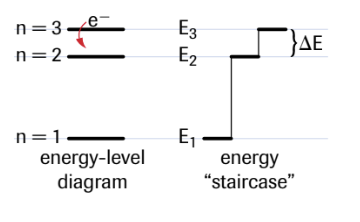
\includegraphics[width=0.4 \textwidth]{../figures/bohr-model-quantum-numbers.png}
    \caption{Bohr's principle energy levels, designated by $n$, are
        like unequal steps on an energy staircase. If an electron ``falls'' from a higher energy level,
        such as $n=3$, to a lower energy level, such as $n=2$, the difference between the steps is
        released as a photon of light.}
    \label{fig:bohr-model-quantum-numbers}
\end{figure}

\subsection{Secondary Quantum Number}
This represents the shape of the orbital. Denoted by $\ell$, it has the range 
\begin{align*}
    \text{theoretical: }&[0,\,n-1]\\
    \text{practical: }&[0,\,4]\\
    \text{notation }&(s,\,p,\,d,\,f)
\end{align*}
\begin{bulleted-list}
    \item \textbf{Arnold Sommerfeld} expanded on Bohr's theory when he realized many
        of the lines Bohr observed were actually \textbf{multiple lines} very tightly
        together.
    \item Sommerfield decided to split energy levels into \textbf{sub-energy} levels,
        having only slightly different energies. This is how they derived the secondary 
        quantum number. See Figure \ref{fig:sommerfield-model}.
\end{bulleted-list}

\begin{figure}[ht!]
    \centering
    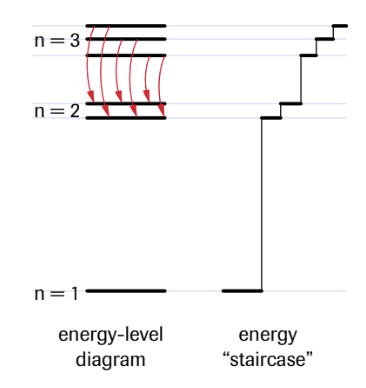
\includegraphics[width=0.4 \textwidth]{../figures/sommerfield-model.png}
    \caption{Sommerfield's model adds more sublevels to all of the Bohr main levels. Compare with
        Figure \ref{fig:bohr-model-quantum-numbers} to see the difference.}
    \label{fig:sommerfield-model}
\end{figure}

\begin{sample}{What is the similarity in the type of observations used by Bohr and Sommerfield?}
    The similarity is that there are main energy levels for the electrons. Both models use
    the principle quantum number to describe the main energy sublevel.
\end{sample}

\begin{sample}{What is the difference in the electron orbits proposed by Bohr and those of
    Sommerfield?}
    Bohr proposed that there was only one energy level, while Sommerfield proposed that there
    were actually many sublevels within each energy level. Sommerfield used the observation that
    the bright-lines in the emission spectrum of hydrogen were actually composed of many more
    lines to create his hypothesis.
\end{sample}

\subsection{Magnetic Quantum Number}
This represents the orientation of the orbital. Denoted
by $m_\ell$, it has the range
\[
    m_\ell\in[-\ell,\,\ell]
\]
\begin{bulleted-list}
    \item If a gas discharge tube is placed near a strong magnet, some single lines split into
        new lines. This is called the \textbf{Zeeman effect}, see Figure \ref{fig:zeeman-effect}.
    \item Sommerfield and Debye's explanation was that orbits could exist at various angles. The
        idea is that if the orbits are oriented in space in different planes, the energies of
        the orbits are different when an atom is near a strong magnet, hence the lines splitting.
\end{bulleted-list}

\begin{figure}[ht!]
    \centering
    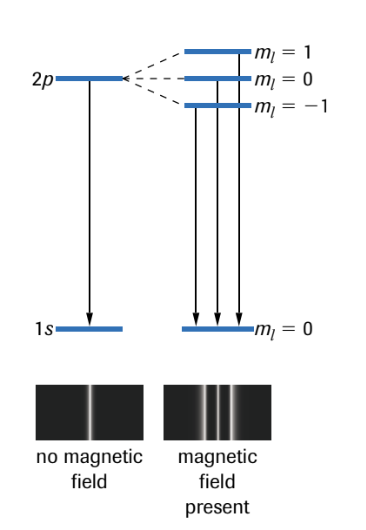
\includegraphics[width=0.4 \textwidth]{../figures/zeeman-effect.png}
    \caption{The triplets in spectra produced in a magnetic field are explained by creating a third
        quantum number, corresponding to the angled orbits in an orbit type}
    \label{fig:zeeman-effect}
\end{figure}

\subsection{Spin Quantum Number}
This represents the spin of the electron in the orbital.
Denoted by $m_s$, it has the range
\[
    m_s\in[-\frac{1}{2},\,+\frac{1}{2}]
\]
Where $+\frac{1}{2}$ corresponds to ``spin up'' and $-\frac{1}{2}$ corresponds to ``spin down''. 
\begin{bulleted-list}
    \item This was introduced because when they experimented with hydrogen, some electrons repelled, and 
        some attracted. Therefore, they concluded that the way the electron must be spinning around the 
        nucleus is different.
    \item Some elements and compounds are \textbf{paramagnetic}, like $\ch{O2_{(\ell)}}$.
    \item The spins are equal in magnitude but opposite in value, hence $\pm\frac{1}{2}$
\end{bulleted-list}

\begin{problems}
    \item What is the main kind of evidence used to develop the description of electrons in terms
        of quantum numbers?
    \item Briefly, what is the theoretical description of electrons in atoms provided by each of
        the four quantum numbers?
    \item Theoretical knowledge in science develops from an need to explain what is observed. What
        is the fourth quantum number and why is it necessary?
    \item If every electron must have a unique set of four quantum numbers, how many different
        electrons can there be for each principle number from $n=1$ to $n=3$?
\end{problems}
\begin{solutions}
    \item Line and continuous spectra is the main kind of evidence used to develop the description
        of electrons in terms of quantum numbers. These spectra are created through the practice
        of spectroscopy.
    \item $n$ represents the energy level, $\ell$ represents the shape of the orbital in the energy level,
        $m_\ell$ represents the orientation of the orbitals, and $m_s$ represents the spin of
        the electron in the orbital.
    \item The fourth quantum number helps explain the paramagnetism traits of some elements and
        compounds. Because the spins are equal in magnitude but opposite in charge, $m_s=\pm\frac{1}{2}$.
    \item There are a maximum of $2n^2$ electrons in a given energy level
        \begin{align*}
            n=1:&\quad2\\
            n=2:&\quad8\\
            n=3:&\quad18
        \end{align*}
\end{solutions}
